\documentclass[tikz,border=10pt]{standalone}
\usepackage{tikz}
\usepackage{pgfplots}
\pgfplotsset{compat=1.18}
\usetikzlibrary{arrows.meta, calc}

\begin{document}
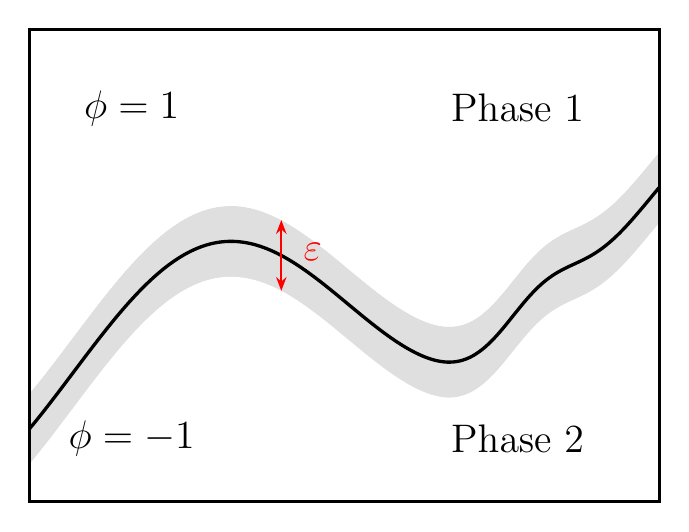
\begin{tikzpicture}

    % --- Dimensions ---
    \def\BoxW{8}
    \def\BoxH{6}
    \def\EpsHalf{0.45}  % half-width of interface band

    % --- Outer Box ---
    \draw[very thick, fill=white] (0,0) rectangle (\BoxW,\BoxH);

    % --- Define the boundary curve function ---
    % f(x) = 1.5 + 0.25*x + 1.2*sin(0.9*x - 0.5) + 0.6*exp(-((x-6.5)^2)/0.5)
    % In pgfplots degrees mode for sin: convert to deg
    % Actually we use TikZ plot with gnuplot-style or pgfplots

    % --- Gray interface band (fill between upper and lower boundary) ---
    % Upper boundary
    \fill[gray!25]
        plot[domain=0:\BoxW, samples=200, smooth]
            ({(\x)}, {1.5 + 0.25*(\x) + 1.2*sin(0.9*(\x) r - 0.5 r) + 0.6*exp(-((\x)-6.5)*((\x)-6.5)/0.5) + \EpsHalf})
        -- (\BoxW, 0) -- (0, 0) -- cycle;

    % Now cover below the lower boundary with white to create the band effect
    \fill[white]
        plot[domain=0:\BoxW, samples=200, smooth]
            ({(\x)}, {1.5 + 0.25*(\x) + 1.2*sin(0.9*(\x) r - 0.5 r) + 0.6*exp(-((\x)-6.5)*((\x)-6.5)/0.5) - \EpsHalf})
        -- (\BoxW, 0) -- (0, 0) -- cycle;

    % Also need to cover above the upper boundary with white (to clip to box)
    \fill[white]
        plot[domain=0:\BoxW, samples=200, smooth]
            ({(\x)}, {1.5 + 0.25*(\x) + 1.2*sin(0.9*(\x) r - 0.5 r) + 0.6*exp(-((\x)-6.5)*((\x)-6.5)/0.5) + \EpsHalf})
        -- (\BoxW, \BoxH) -- (0, \BoxH) -- cycle;

    % Redraw the white region above upper boundary so it's clean
    % (this approach: fill gray below upper, then white below lower)

    % --- The main boundary curve (black line) ---
    \draw[black, very thick]
        plot[domain=0:\BoxW, samples=200, smooth]
            ({(\x)}, {1.5 + 0.25*(\x) + 1.2*sin(0.9*(\x) r - 0.5 r) + 0.6*exp(-((\x)-6.5)*((\x)-6.5)/0.5)});

    % --- Redraw outer box border (may have been covered by fills) ---
    \draw[very thick] (0,0) rectangle (\BoxW,\BoxH);

    % --- Labels ---
    % Phase 1 (upper region, phi = 1)
    \node[font=\Large] at (1.3, 5.0) {$\phi = 1$};
    \node[font=\Large] at (6.2, 5.0) {Phase 1};

    % Phase 2 (lower region, phi = -1)
    \node[font=\Large] at (1.3, 0.8) {$\phi = -1$};
    \node[font=\Large] at (6.2, 0.8) {Phase 2};

    % --- Epsilon annotation (red double arrow) ---
    % Place at x=3.2, compute y values for upper and lower bands
    % At x=3.2: f(3.2) = 1.5 + 0.8 + 1.2*sin(2.88-0.5 rad) + 0.6*exp(-((3.2-6.5)^2)/0.5)
    % sin(2.38 rad) ~ 0.674 => 1.2*0.674 ~ 0.81
    % exp(-21.78/0.5) ~ 0 (negligible)
    % f(3.2) ~ 1.5 + 0.8 + 0.81 = 3.11
    % So arrow from 3.11 - 0.45 = 2.66 to 3.11 + 0.45 = 3.56

    \pgfmathsetmacro{\arrowX}{3.2}
    \pgfmathsetmacro{\fval}{1.5 + 0.25*\arrowX + 1.2*sin(0.9*\arrowX r - 0.5 r) + 0.6*exp(-(\arrowX-6.5)*(\arrowX-6.5)/0.5)}
    \pgfmathsetmacro{\arrowBot}{\fval - \EpsHalf}
    \pgfmathsetmacro{\arrowTop}{\fval + \EpsHalf}

    \draw[red, thick, {Stealth[length=5pt]}-{Stealth[length=5pt]}]
        (\arrowX, \arrowBot) -- (\arrowX, \arrowTop);

    \node[red, font=\Large] at ({\arrowX + 0.4}, {\fval + 0.05}) {$\varepsilon$};

\end{tikzpicture}
\end{document}
